Architectural decisions often exhibit complex and cross-cutting 
impacts upon the design, therefore communicating this information textually or socially can be quite challenging. Archie's visualization feature helps developers understand underlying design decisions within the context of the design and/or code. This can be especially helpful in agile projects where~\emph{no time for training} is a common occurrence~\cite{SEI_MaximumAwesome_url}  and design knowledge is primarily shared through social mechanisms such as pair-programming and regular meetings. When using Archie, a developer can automatically generate a view of the system illustrating tactics implemented in the source code and the files involved in the implementation.

\begin{figure}[tbph]
\centering
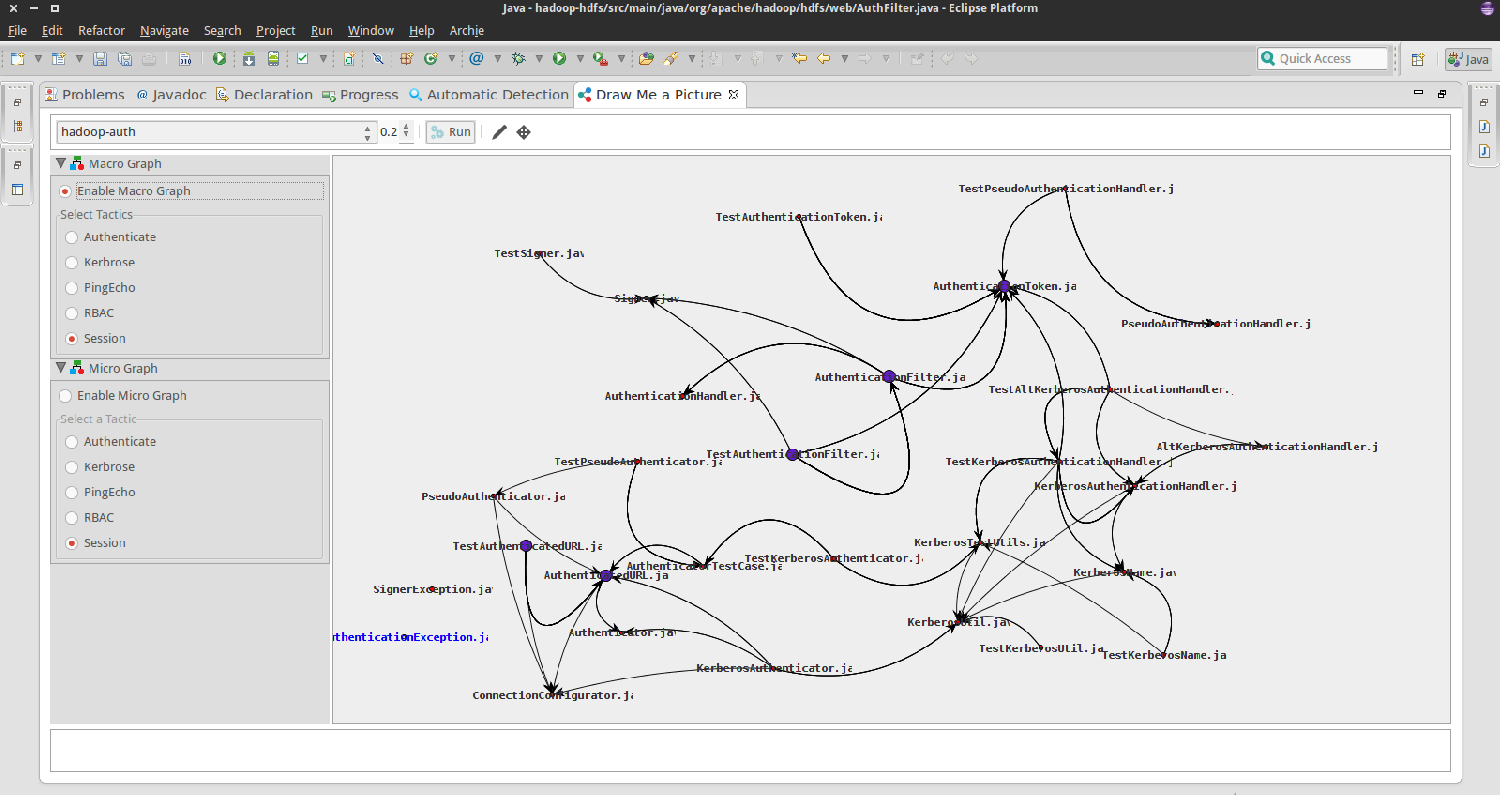
\includegraphics[width=0.9\linewidth]{./Visual1}
\caption{Visualization of Secure Session Management tactic Hadoop HDFS }
\label{fig:Visual1}
\end{figure}

Figure~\ref{fig:Visual1} depicts an automated visualization of secure session tactic in Hadoop HDFS subsystem. This view shows the source files involved in the implementation of tactic. In another example (Figure~\ref{fig:Audit}), we illustrate how Audit Trail tactic is implemented in Hadoop HDFS project, as well as the test files implemented to test this tactic. 

\begin{figure}[tbph]
\centering
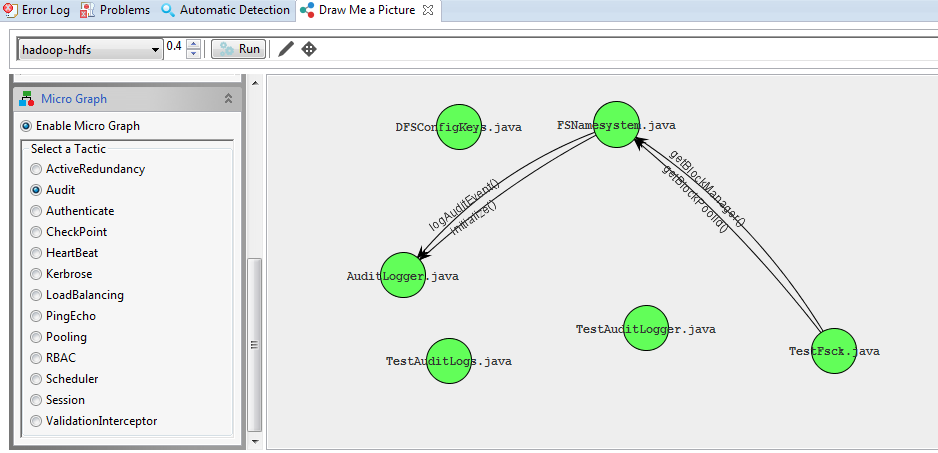
\includegraphics[width=0.9\linewidth]{./Audit}
\caption{Visualization of Audit Trail tactic and related test cases in Hadoop HDFS}
\label{fig:Audit}
\end{figure}
 

Archie provides features to help developers quickly create actionable models of tactical spikes. In this scenario, a developer may use Archie's automatic detection engine to locate implemented tactical spikes, and then connect these code snippets into TTPs. Establishing connections between source files and elements of TTPs requires only a single click. These features provide an easy and fast approach for creating rich architectural models during development. Furthermore, since these models are integrated with source code, any new programmer can open them in the programming IDE and understand the design decisions behind the code, the driving requirements, and the rationales behind design choices. Since TTPs can be customized, developers can add their own notes and elements into the model and communicate it with other developers on the team.